%\AtBeginDocument{\RenewCommandCopy\qty\SI}
\documentclass[uplatex]{jsbook}

\usepackage{amsmath,amssymb}
\usepackage{mathtools}
\usepackage{physics}
\usepackage[separate-uncertainty=true]{siunitx}
\usepackage[dvipdfmx]{graphicx}
\usepackage[dvipdfmx]{color}
\usepackage[left=2cm,right=2cm,top=2cm,bottom=2cm,twoside]{geometry}
%\usepackage{fancyhdr}
%\pagestyle{fancy}
%\lhead{\leftmark}{\leftmark}
%\rhead{\rightmark}{\rightmark}
\renewcommand{\labelenumi}{(\arabic{enumi})}
\newcommand{\rot}{\curl}
\makeatletter
\@addtoreset{equation}{section}
\def\theequation{\thesection.\arabic{equation}}% renewcommand でもOK
\makeatother

%\usepackage{lineno}
%\linenumbers
\usepackage{url}
\usepackage{here}
\usepackage{hyperref}
\usepackage{breakurl}
\usepackage{subcaption}
\usepackage{comment}
\usepackage{caption}
\captionsetup[table]{justification=centering}
\captionsetup[figure]{justification=centering}

\makeatletter
\newcommand{\figcaption}[1]{\def\@captype{figure}\caption{#1}}
\newcommand{\tblcaption}[1]{\def\@captype{table}\caption{#1}}
\makeatother



\begin{document}
\frontmatter
\begin{titlepage}%
    \makeatletter
    \let\footnotesize\small
    \let\footnoterule\relax
    \let\footnote\thanks
    \null\vfil
    \vskip 20\p@
    \begin{center}%
      {\large 筑波大学 理工学群 物理学類\par}%
      {\large 卒業論文\par}%
      \vskip 12em%
      {\LARGE
        \begin{tabular}[t]{c}%
          高い時間分解能を持つAC-LGAD検出器の\\増幅率および時間分解能の研究
        \end{tabular}\par}%
      \vskip 25em%
      {\large
        \begin{tabular}[t]{r}%
          令和6年1月\\
        \end{tabular}%
          \vskip 0.5em%
        \begin{tabular}{r}
          学籍番号 202012130\\           
        \end{tabular}%
          \vskip 0.5em%
        \begin{tabular}{r}
          著者氏名 堀越一生\\
        \end{tabular}
          \vskip 0.5em%
        \begin{tabular}{r}
          指導教員 廣瀬茂輝
        \end{tabular}\par}%
      \end{center}
    \par
    \@thanks\vfil\null
    \makeatother
  \end{titlepage}%    %*** 表紙のファイル

\newpage
\thispagestyle{empty}
~
\newpage

\thispagestyle{empty}
\begin{center}
  {\Large 〇〇論文 202X年度(令和X年度)}

  {\LARGE 論文タイトル\\改行も可能}
\end{center}

\quad

\begin{flushright}
    学籍番号 名前

    指導教員 先生の名前
\end{flushright}

\quad

{\large \gt 論文要旨}

%\begin{comment}
  標準理論を超える物理現象や新粒子を発見するために、加速器実験は高輝度化と高エネルギー化を繰り返しながら発展してきた。
  こんな感じで論文要旨を書ける。


%\end{comment}
    %*** 概要のファイル

\pagestyle{headings}
\setcounter{tocdepth}{2}
\tableofcontents
\listoffigures
\listoftables

\mainmatter

  %*** Chapter 1
  \chapter{背景}
  \section{新粒子の探索}
粒子をぶつけて新粒子の探索を行っている。


  \section{大型加速器実験}
加速器実験では、加速させた高エネルギーの粒子同士を衝突させることで、新たな粒子を作り出すことや、粒子同士の相互作用を観測することができる。

LHCは、図\ref{fg:LHC}にあるように1 周約27 kmの加速器である。

\begin{figure}[h]  %*** 図の挿入方法
    \centering
    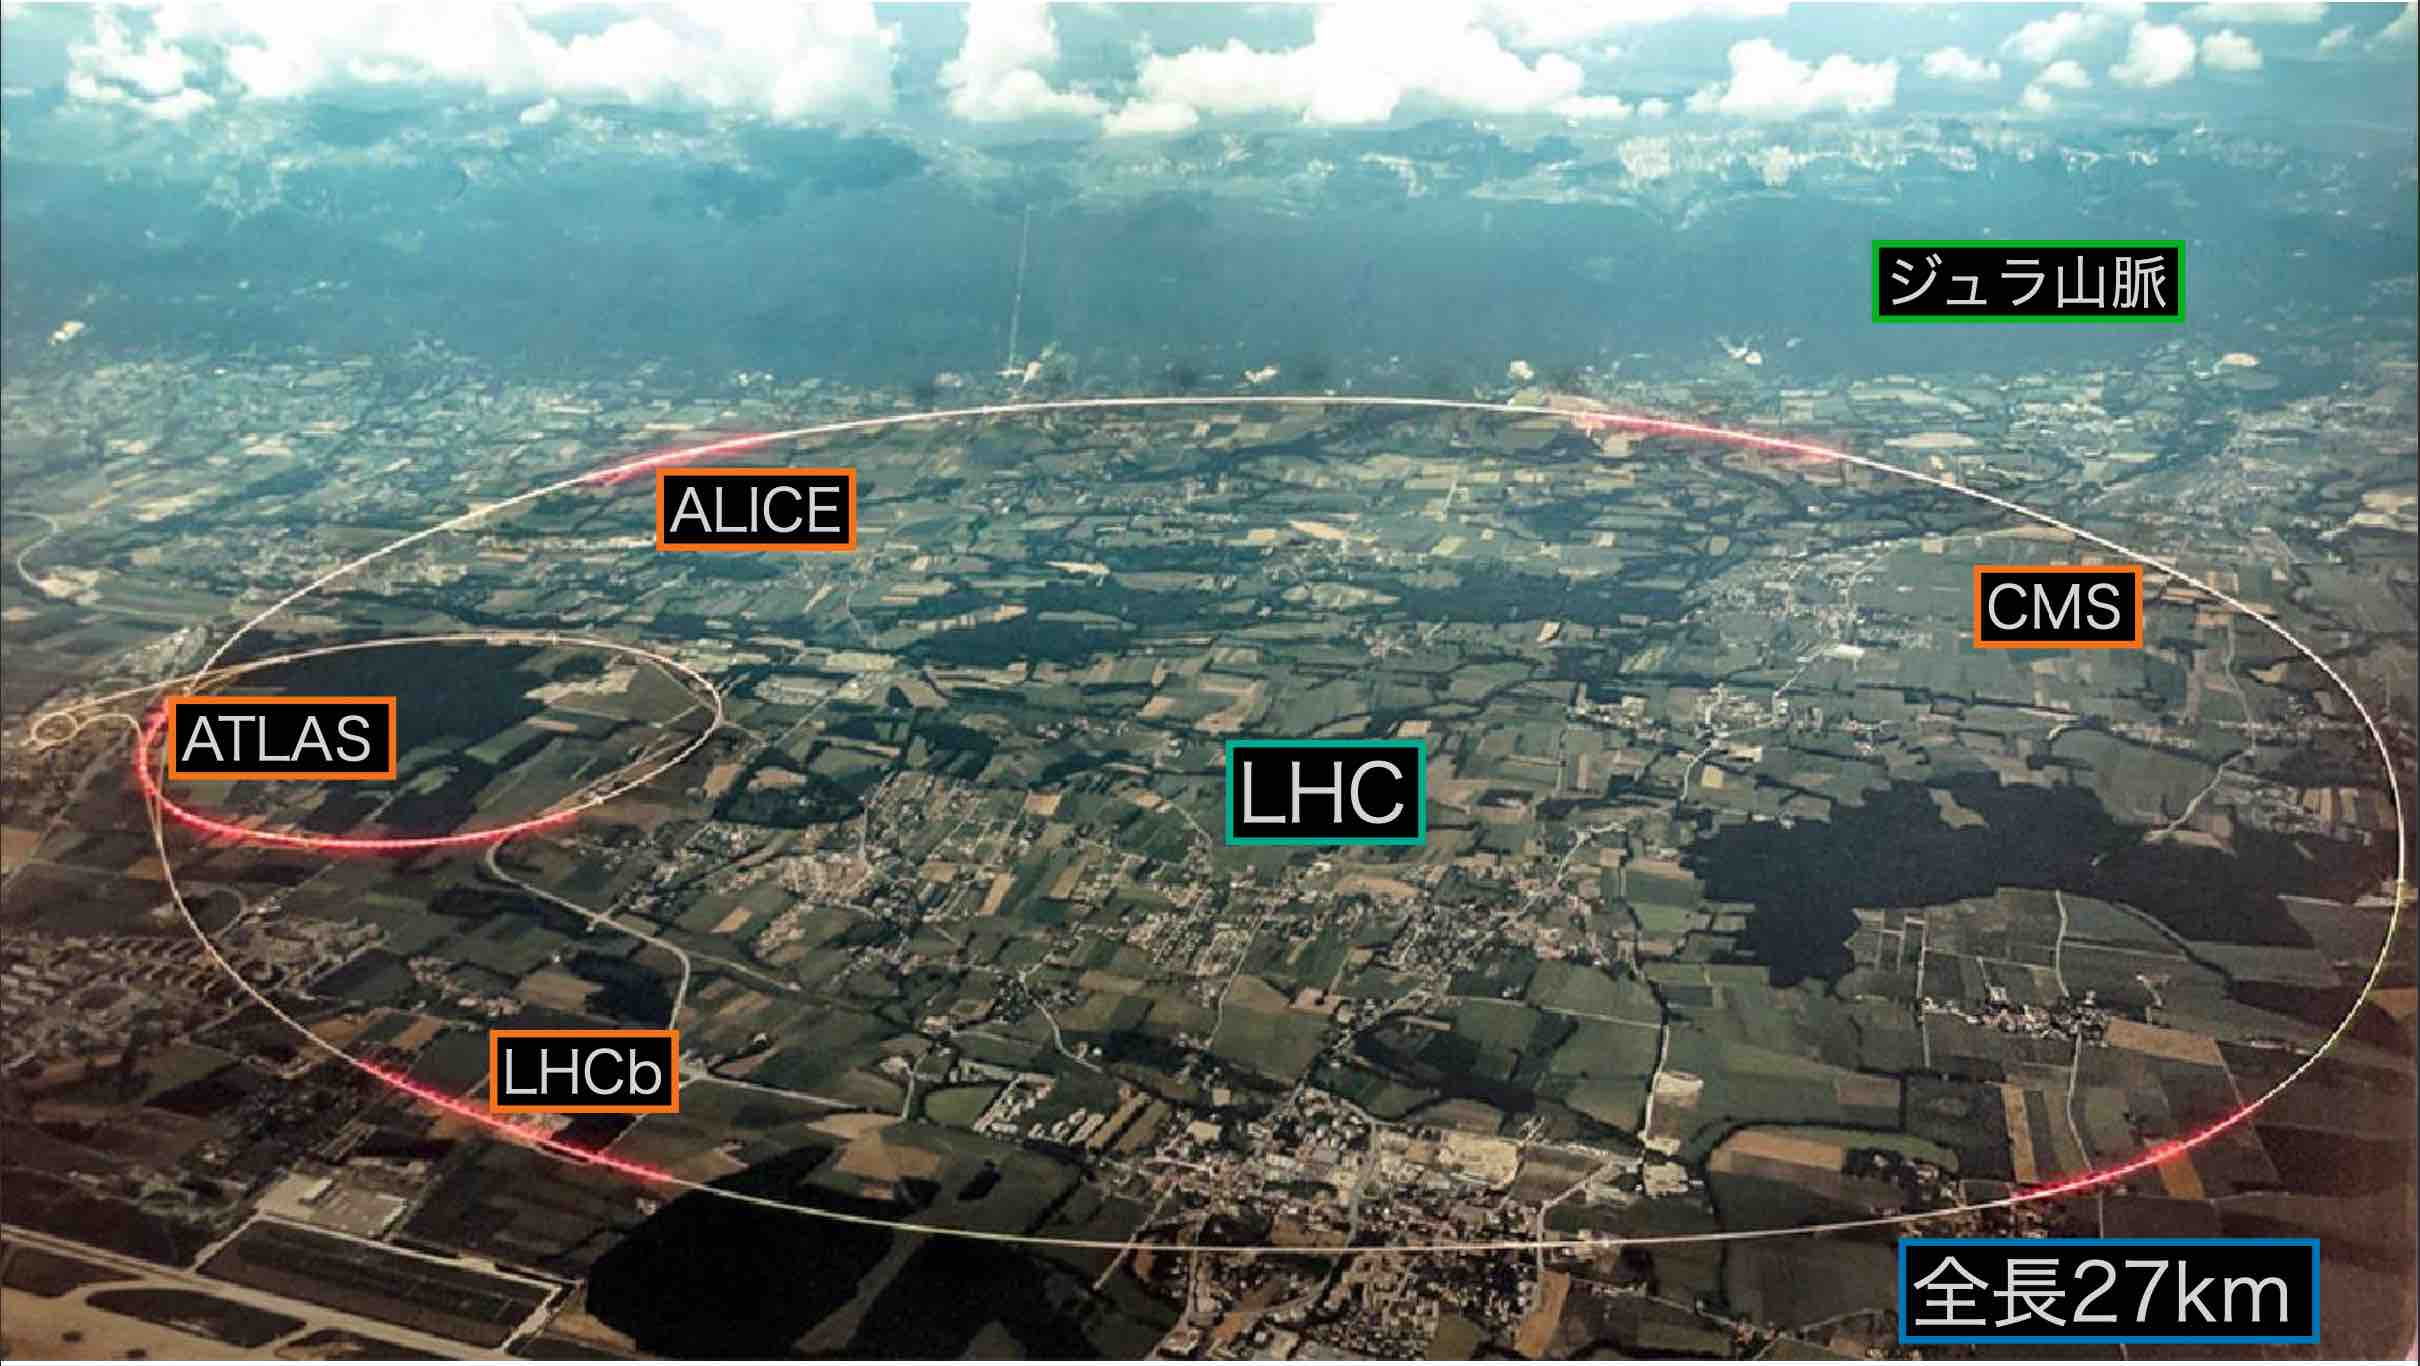
\includegraphics[width=12cm]{fig/ch1/LHC.jpg}
    \caption{Large Hadron Colider(LHC)の鳥瞰図\cite{LHCphoto}}
    \label{fg:LHC}
\end{figure}
  \section{内部飛跡検出器}
%内部飛跡検出器は、加速器実験の衝突点を複数層に囲むようにして設置される粒子検出器の中で、最内層に設置される検出器である。
内部飛跡検出器は、検出器内に荷電粒子が通過すると、検出器内で電子正孔対が生成され、通過した情報として電気信号を出力することができる。
そのため、検出器に粒子が通過した情報を元に、粒子の飛跡を再構成することができる。
%粒子の飛跡からビームの衝突点、磁場による飛跡の曲率から粒子の運動量を測定することができる。
%測定から得られた情報から、衝突によって生成された粒子の性質や相互作用について調べることができる。

\begin{figure}[h]
    \centering
    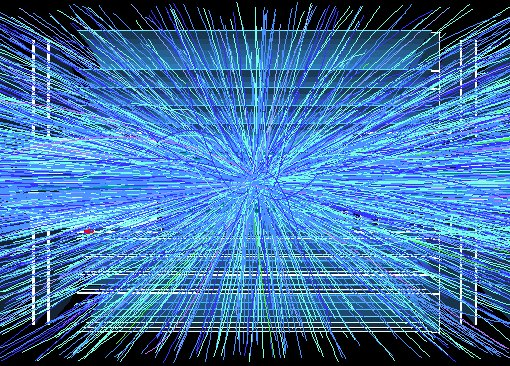
\includegraphics[width=10cm]{fig/ch1/HL-LHC_simulation.jpeg}
    \caption{HL-LHCの衝突点の様子\cite{HL-LHCsimulation}}
    \label{fg:HL-LHCsimulation}
\end{figure}

将来の加速器実験では、生成確率が低い粒子や質量が大きい粒子を発見するために、重心系エネルギーと衝突頻度を向上させる計画が検討されている。
加速器によって加速される粒子は、バンチと呼ばれる粒子の塊となっており、加速器実験ではその塊を衝突させている。
データ量の増加には、1バンチに含まれる粒子数を増やすことで衝突点の数を多くすることや、バンチとバンチの間隔を縮めて、衝突の頻度を高くすることが有効である。
現在のLHCでは1回のバンチ交差あたり最大60個の衝突が起きるが、
図\ref{fg:HL-LHCsimulation} のHL-LHCにおける衝突点のシミュレーション\cite{HL-LHCsimulation}では、
1バンチで200回の陽子-陽子衝突が生じるとシミュレーションされている。
HL-LHCに限った話ではなく、将来の加速器実験を見据えた際には、さらなる衝突回数の増加があると考えられる。
粒子の衝突によって生じる事象のほとんどが背景事象で、その中から調べたい衝突を見つけなければならない。
内部飛跡検出器には大量の粒子が通過するため、その情報から粒子1つ1つの飛跡を再構成できるような性能が求められる。
加速器の高輝度化に対応できる内部飛跡検出器の開発が必要不可欠である。

HL-LHC実験で使われるATLAS検出器では、主に電極サイズが$50 \mu\rm{m}$×$50 \mu\rm{m}$のピクセル検出器を使用する。
検出器の電極サイズを細かくすることで、位置分解能を向上とoccupancyを下げることができるため、
多数の衝突から生成される粒子の飛跡をより確実に再構成できる。
高い位置分解能に加えて、検出器に高い時間分解能を持たせることで粒子の飛跡に時間情報を追加することができる。
図\ref{fg:4DTracking} に位置情報と時間情報を用いて飛跡を再構成した様子を示す。
\begin{figure}[h]
    \centering
    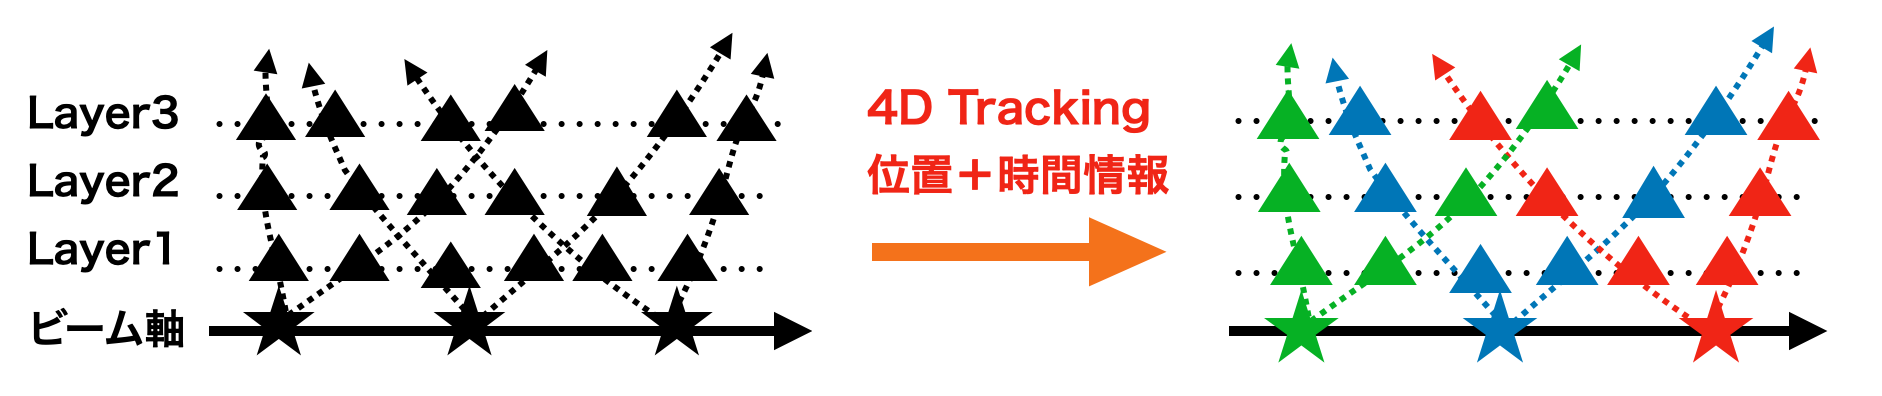
\includegraphics[width=16cm]{fig/ch1/4DTracking_new.png}
    \caption[位置情報と時間情報による飛跡の再構成の様子]{位置情報と時間情報による飛跡の再構成の様子。星印が粒子のヒット情報で点線が再構成した飛跡である。\\時間分解能を持たせた検出器を用いることで、飛跡と衝突点を時間で区別することができる様子を示している。}
    \label{fg:4DTracking}
\end{figure}
星印が衝突点で、三角が粒子のヒット情報である。
検出器が3層に設置されており、ビーム軸上で起きた衝突から3つの検出器がヒット情報を得ることで、飛跡を再構成した様子点線が再構成した飛跡である。
左の図が時間情報のない場合で、右の図が時間情報がある場合の様子である。
時間情報があることで、飛跡の再構成することに加えて、右の図で衝突点と飛跡を色で区別したように、時間で区別することが可能になる。

図\ref{fg:4Dtrack_ATLAS} には、HL-LHCのATLAS実験による衝突点のシミュレーション結果を示す\cite{ATL-PHYS-PUB-2023-023}。
左の図が位置分解能による飛跡の再構成で、右の図が位置分解能と時間分解能による飛跡の再構成を示している。
時間分解能が加わることによって、衝突点と飛跡の時間情報の取得により、粒子密度が高い状況でも高輝度化に伴うパイルアップによって困難とされる、飛跡の再構成が可能となる。
1 cm単位で検出器を設置する場合、光速で進む粒子の飛跡に時間情報を加えるためには、30 psの時間分解能を満たす必要がある。
加速器の高輝度化に対して、高い時間分解能と位置分解能を併せ持つ内部飛跡検出器が非常に有効であり、新粒子や新物理の発見に大きく貢献することができる。

\begin{figure}[h]
    \begin{minipage}[b]{0.5\linewidth}
        \centering
        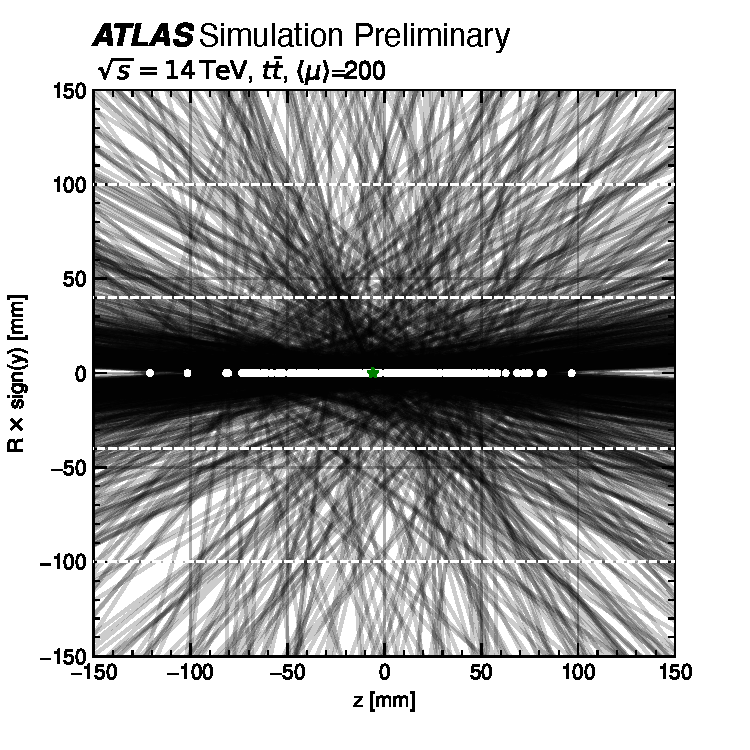
\includegraphics[scale=0.5]{fig/ch1/ATLAS_3Dtrack.pdf}
        \subcaption{位置分解能による飛跡の再構成}
        \label{fg:ATLAS_3Dtrack}
    \end{minipage}
    \begin{minipage}[b]{0.5\linewidth}
        \centering
        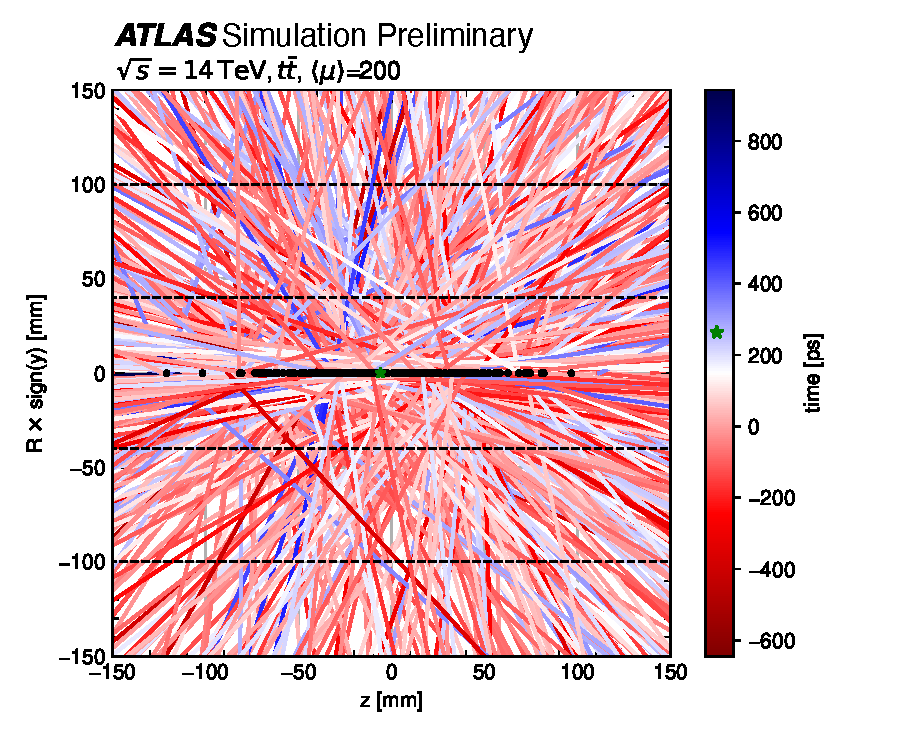
\includegraphics[scale=0.5]{fig/ch1/ATLAS_4Dtrack.pdf}
        \subcaption{位置分解能と時間分解能による飛跡の再構成}
        \label{fg:ATLAS_4Dtrack}
    \end{minipage}
    \caption[飛跡の再構成のシミュレーション\cite{ATL-PHYS-PUB-2023-023}]{飛跡の再構成のシミュレーション\cite{ATL-PHYS-PUB-2023-023}\\時間分解能があることで、衝突点と飛跡がどのタイミングで起こったのかがわかる。粒子密度が高くなっても衝突点と飛跡の紐付けが可能。}
    \label{fg:4Dtrack_ATLAS}
\end{figure}



 
  %*** Chapter 2
  \chapter{LGAD検出器の原理}
  \section{半導体とシリコン検出器}
\subsection{$pn$接合}
$p$型半導体と$n$型半導体を接合させた時の接触した領域を$pn$接合と呼ぶ。
$pn$接合が形成されると、$p$側と$n$側で電子と正孔の密度差が生じるため、 図\ref{fg:pn} のように
$n$型半導体の電子は$p$型半導体へ拡散し、$p$型半導体の正孔は$n$型半導体へ拡散する。
拡散した電子と正孔が再結合することで、$pn$接合付近にキャリアが少ない領域が形成される。この領域を空乏層という。
$p$側では正孔が拡散し負電荷のアクセプタイオンが中和されずに接合近傍に残る。$n$側では電子が拡散し正電荷のドナーイオンが接合近傍に残る。
これによって空乏層内に、$n$側から$p$側の方向に電界が生じる。この電位を内蔵電位と呼ぶ.

シリコン半導体の空乏層幅$W$は、電荷量を$q$、シリコンの誘電率を$\epsilon_s$、内蔵電位を$V_{\rm{bi}}$、アクセプタイオン濃度$N_{\rm{A}}$、ドナーイオン濃度$N_{\rm{D}}$を使って、
式\ref{eq:bulk} で表すことができる\cite{sze2012semiconductor}。
\begin{equation}
    W = \sqrt{\frac{2\epsilon_{\rm{s}}}{q}\left(\frac{N_{\rm{A}}+N_{\rm{D}}}{N_{\rm{A}} N_{\rm{D}}}\right)V_{\rm{bi}}}
    \label{eq:bulk}
\end{equation}

\begin{figure}[h]
    \centering
    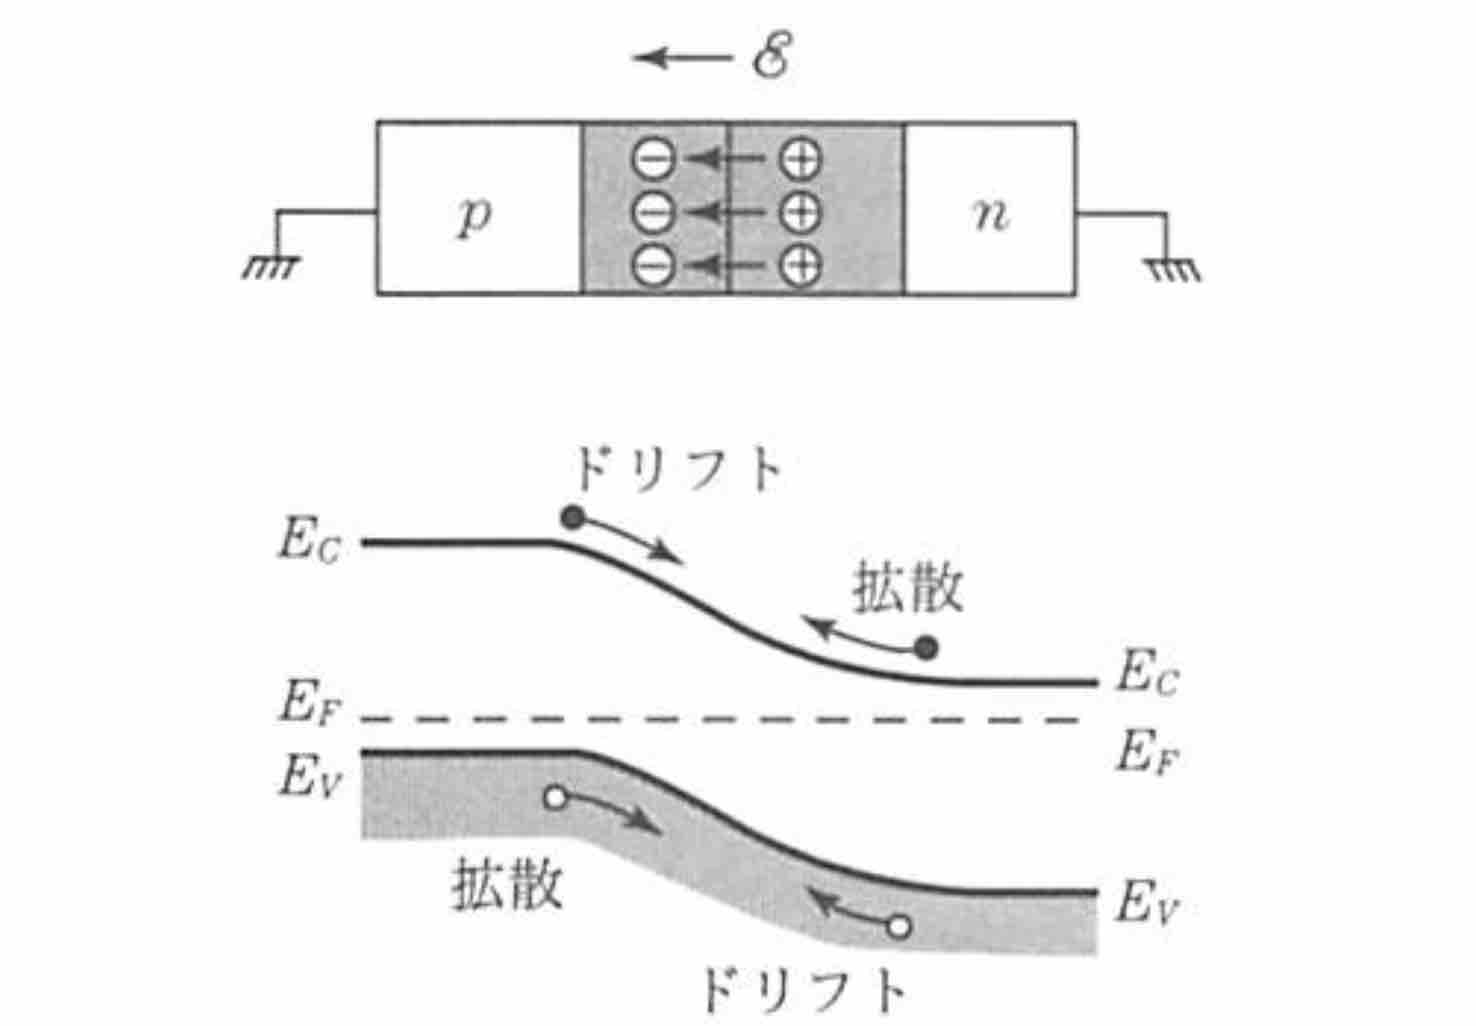
\includegraphics[width=6cm]{fig/ch2/pn.jpg}
    \caption[$pn$接合による電界形成の様子\cite{sze2012semiconductor}]{$pn$接合による電界形成の様子\cite{sze2012semiconductor}\\$n$型半導体の電子と$p$型半導体の正孔が拡散し、$n$側から$p$側へ電界が生じる。}
    \label{fg:pn}
\end{figure}

図\ref{fg:pn_bias} の(a)に$pn$接合の熱平衡状態の空乏層幅とエネルギーバンド図を示す。
空乏層幅が$W$で、$pn$接合のバンドギャップは電荷量を$q$、内蔵電位を$V_{\rm{bi}}$とすると$qV_{\rm{bi}}$と表せる。

\subsubsection{pn接合へ順バイアス電圧の印加}
$pn$接合の$p$側に順バイアス電圧を印加した時の空乏層の様子を 図\ref{fg:pn_bias} の(b)に示す。
$p$側へ$V_{\rm{F}}$の順バイアス電圧を印加すると、$pn$接合の電位は$V_{\rm{F}}$だけ下がるため、空乏層幅は 式\ref{eq:bulk} から減少することがわかる。
$pn$接合のバンドギャップも$q(V_{\rm{bi}}-V_{\rm{F}})$となり熱平衡状態のバンドギャップと比べて減少する。

\subsubsection{pn接合へ逆バイアス電圧の印加}
$pn$接合の$p$側に逆バイアス電圧を印加した時の空乏層の様子を 図\ref{fg:pn_bias} の(c)に示す。
$p$側へ$V_{\rm{R}}$の逆バイアス電圧を印加すると、pn接合の電位は$V_{\rm{R}}$だけ上昇するため、空乏層幅は 式\ref{eq:bulk} から増加することがわかる。
$pn$接合のバンドギャップも$q(V_{\rm{bi}}+V_{\rm{R}})$となり熱平衡状態のバンドギャップと比べて増加する。

\begin{figure}[h]
    \centering
    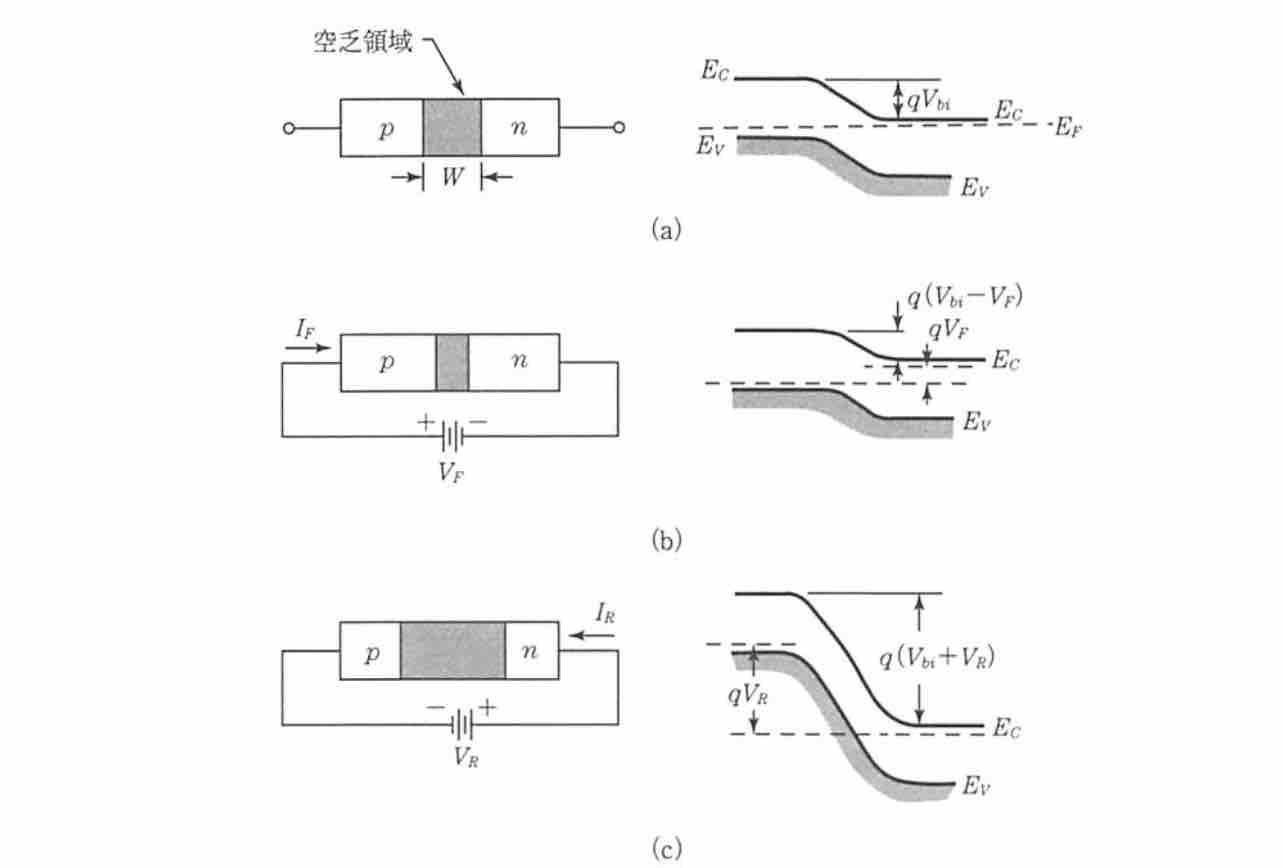
\includegraphics[width=12cm]{fig/ch2/pn_bias.jpg}
    \caption[熱平衡状態、順バイアス電圧、逆バイアス電圧におけるバルクの空乏層幅とエネルギーバンド図\cite{sze2012semiconductor}]{熱平衡状態、順バイアス電圧、逆バイアス電圧におけるバルクの空乏層幅とエネルギーバンド図\cite{sze2012semiconductor}\\(a)が熱平衡状態、(b)が順バイアス電圧、(c)が逆バイアス電圧の様子。}
    \label{fg:pn_bias}
\end{figure}

\subsection{電流電圧特性}
$pn$接合は特定の方向にだけ電流が流れやすい性質を持つ。
図\ref{fg:IV} に$pn$接合の電流電圧特性を示す。
$pn$接合に順バイアス電圧をかけると、$pn$接合のバンドギャップが減少し、キャリアがバンドギャップを越えることが容易になるため、電圧の増加とともに電流が急速に増加する。
逆バイアス電圧をかけると、$pn$接合のバンドギャップが増加するため、キャリアによる電流は流れない。
ある逆バイアスがある電圧に達すると大電流が流れる。
この電圧を降伏電圧と呼び、この電流は電子雪崩によって生じる電流である。

\begin{figure}[h]
    \centering
    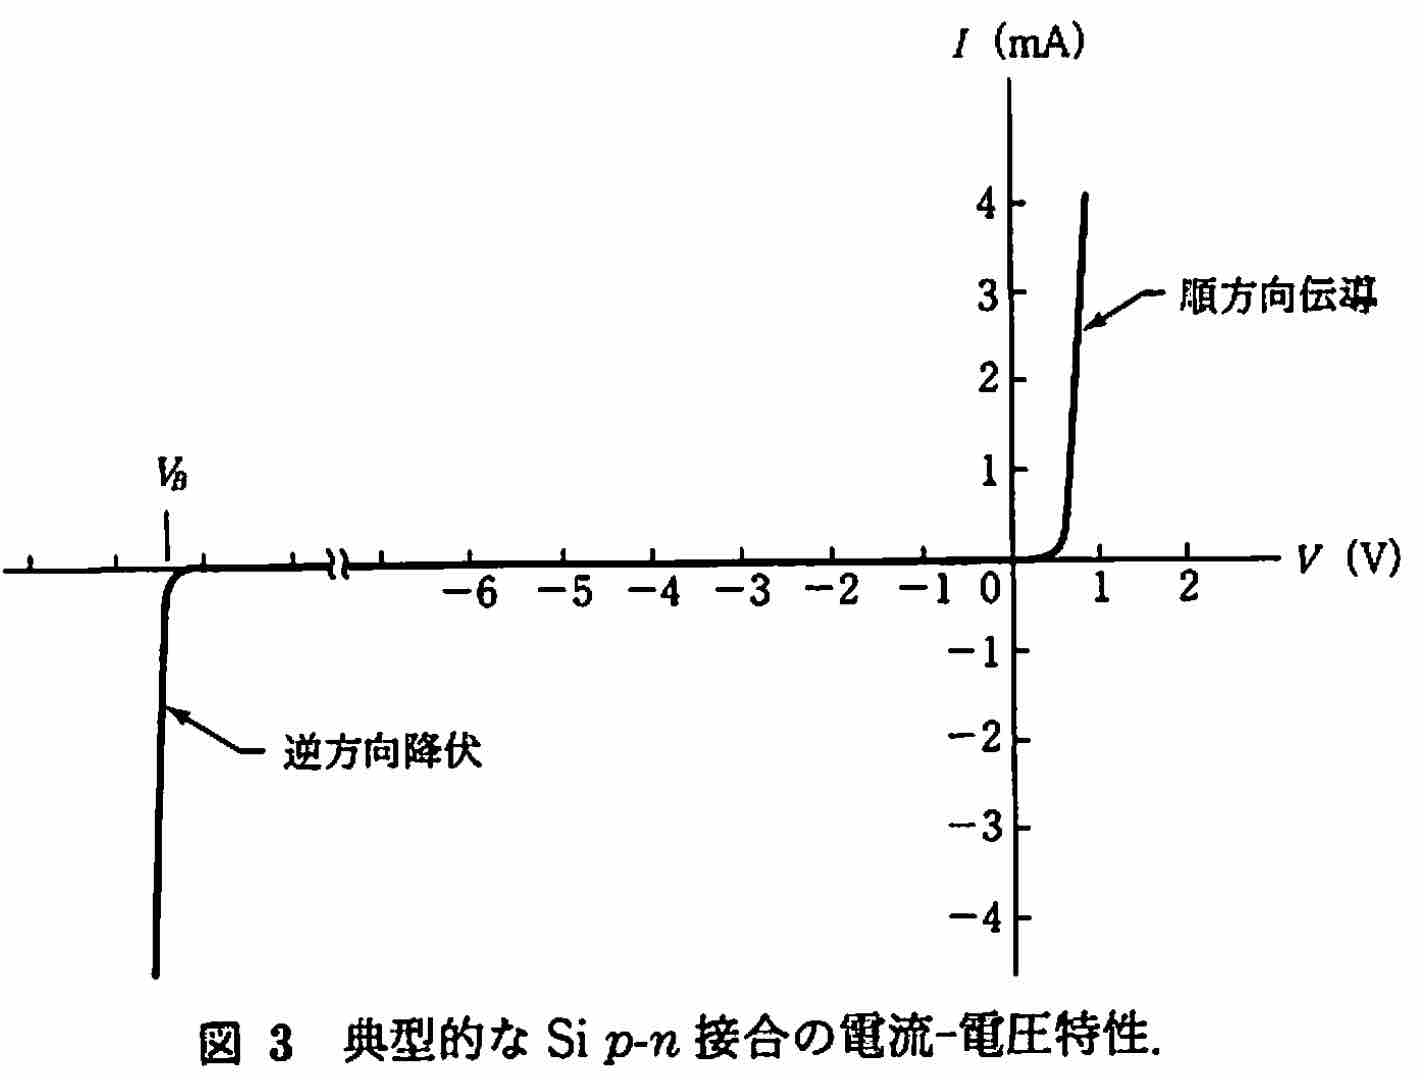
\includegraphics[width=8cm]{fig/ch2/IV.jpg}
    \caption[$pn$接合の電流電圧特性\cite{sze2012semiconductor}]{$pn$接合の電流電圧特性\cite{sze2012semiconductor}\\順バイアス電圧をかけると電圧上昇に伴い電流が上昇し、逆バイアス電圧をかけると降伏電圧で電流が上昇する。}
    \label{fg:IV}
\end{figure}




  \subsection{雪崩増幅}
半導体内の電場がある値を超えると、電子と正孔が雪崩増幅を起こす。図\ref{fg:avalance} はその過程を示したものになっている。
図\ref{fg:avalance} 中の1番の電子に注目すると、高電場によってこの電子の運動エネルギーが増加する。
この電子が格子に衝突した際に、持っていた運動エネルギーによって、格子の結合手を切断し、価電子帯から電子が励起される。
この過程によって生じた電子正孔対が2番の電子と$\rm{2^\prime}$番の正孔である。この電子と正孔も高電場によって、格子に衝突し、電子正孔対を生成する。
このように、高電場によって連鎖的に電子と正孔が生じる過程を電子雪崩(アバランシェ)という。

\begin{figure}[h]
    \centering
    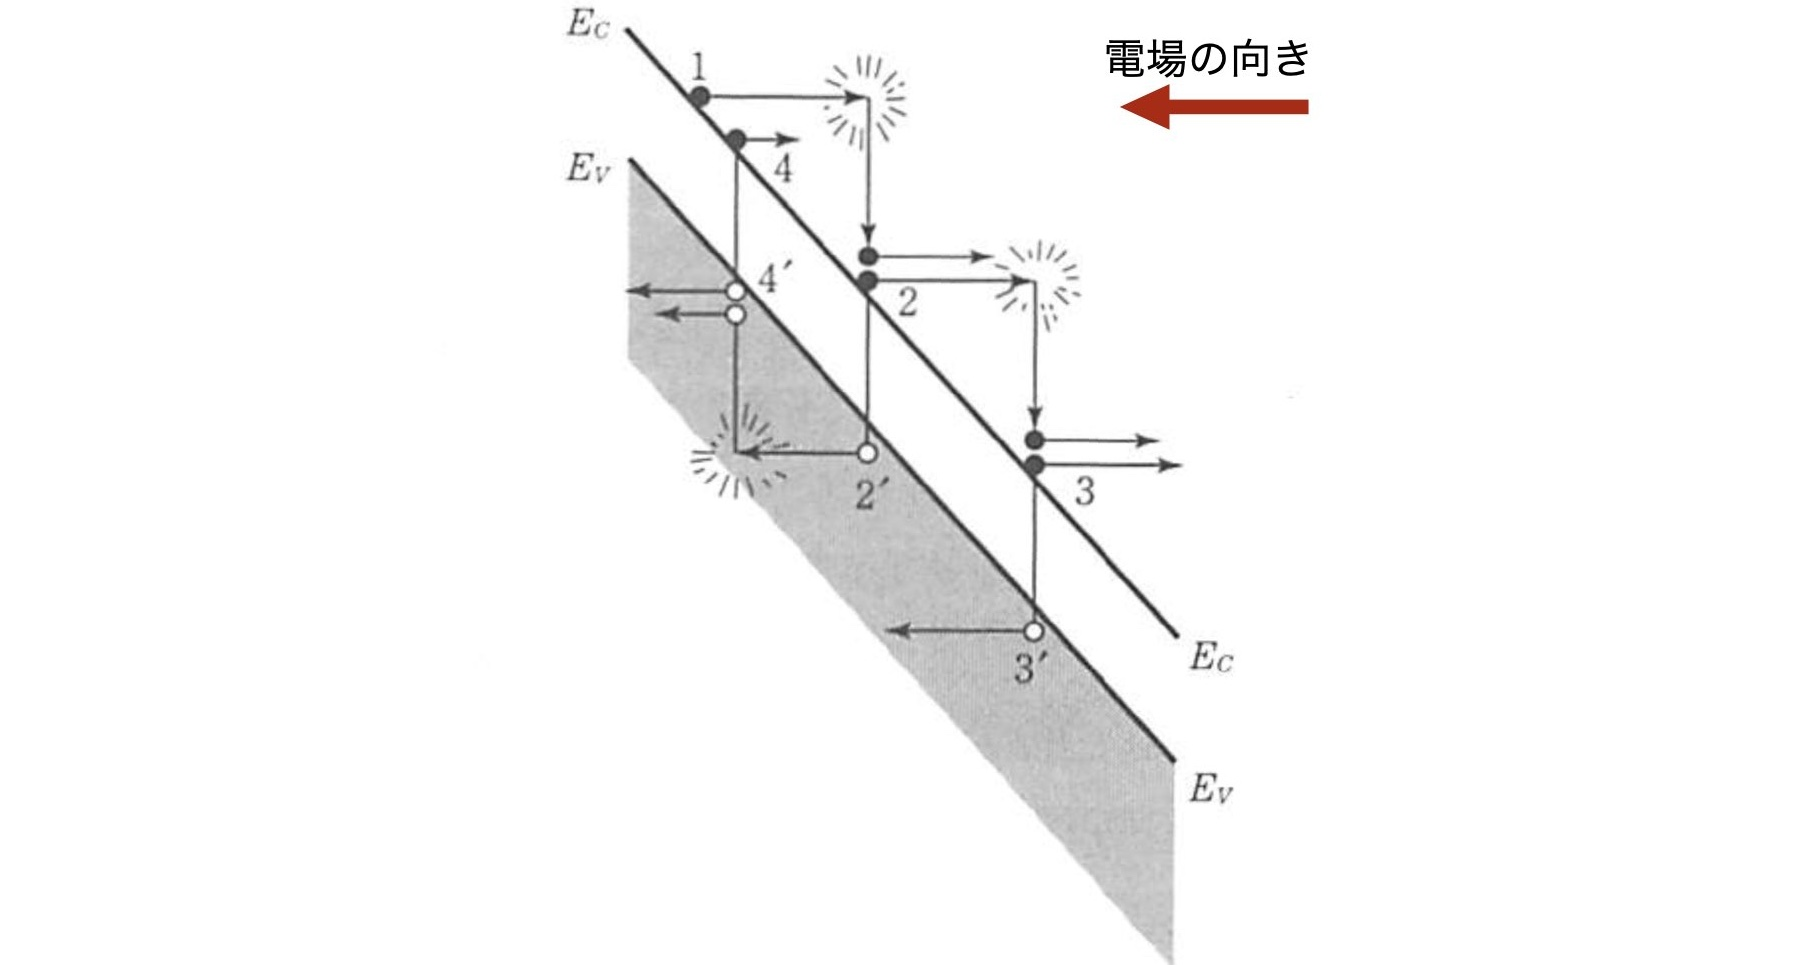
\includegraphics[width=11cm]{fig/ch3/avalance.jpeg}
    \caption[電子雪崩におけるエネルギーバンド図\cite{sze2012semiconductor}]{電子雪崩におけるエネルギーバンド図\cite{sze2012semiconductor}\\電子や正孔が衝突して電子正孔対を生成する現象が繰り返し生じる。}
    \label{fg:avalance}
\end{figure}


  %*** Chapter 3
  \chapter{LGAD検出器の増幅率の測定}
  \section{サンプルの作成}
今回の測定で使用するLGAD検出器は、


  \section{レーザー測定の方法と使用装置}
\subsection{レーザーの性能}
今回のLGAD検出器の増幅率の測定においては、図\ref{fg:Laser} の赤外線パルスレーザーを使用する。
このレーザーは、NKT Photonics社のKATANA 10 \cite{KATANA10}で、レーザーの性能について 表\ref{tab:Laser_performance} にまとめた。

\begin{figure}[h]
    \begin{minipage}[c]{0.45\linewidth}
        \centering
        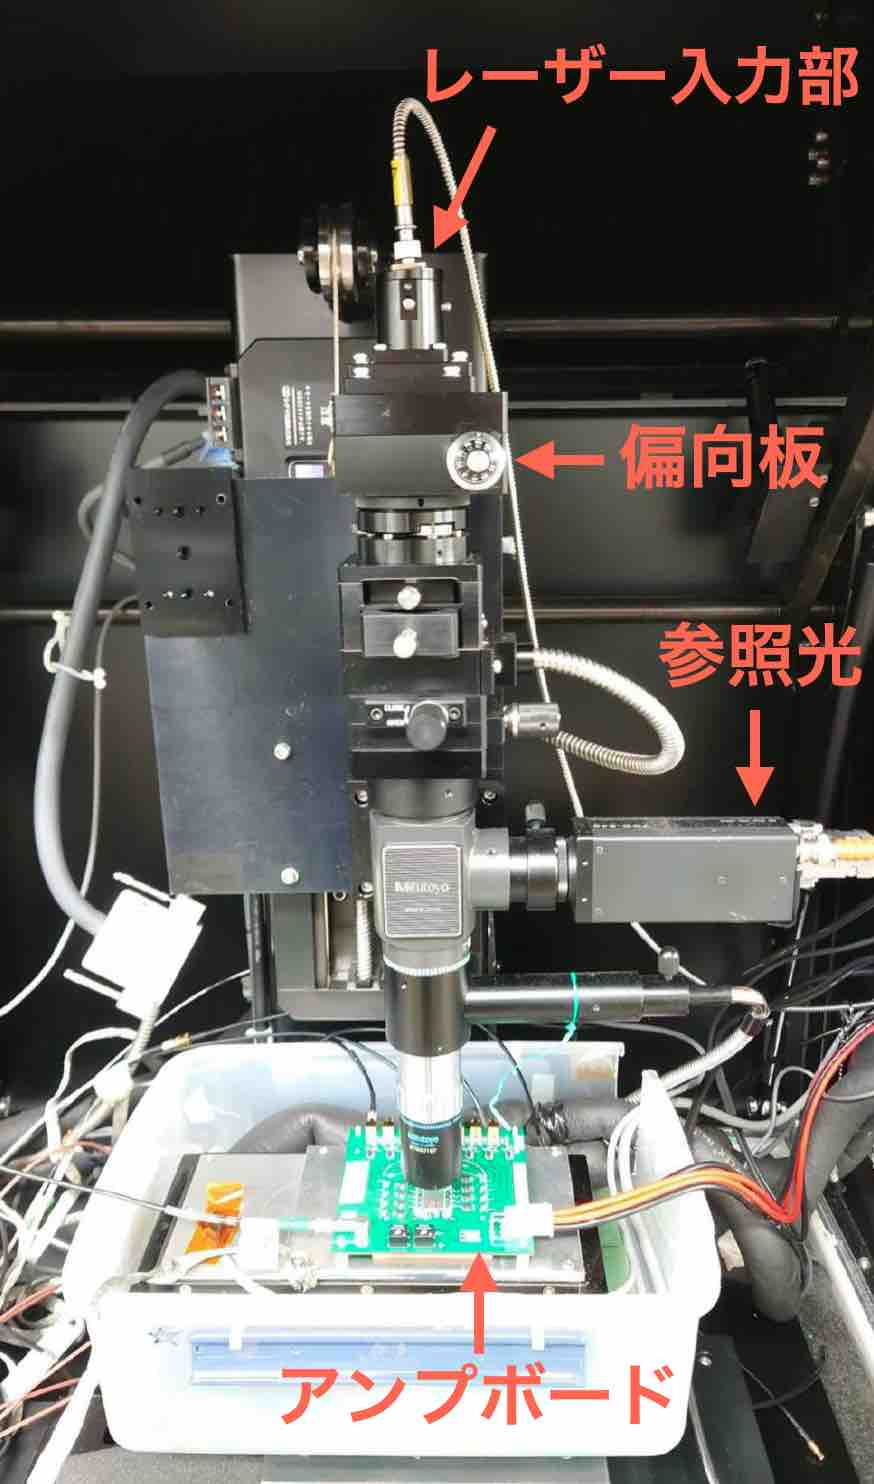
\includegraphics[width=5cm]{fig/ch3/Laser.jpg}
        \caption{赤外線パルスレーザー本体}
        \label{fg:Laser}
    \end{minipage}
    \begin{minipage}[c]{0.45\linewidth}   %*** 表の書き方
        \def\@captype{table}
        \tblcaption{赤外線パルスレーザーの性能表}
        \centering
        \begin{tabular}{cc}
            \hline
            モデル & KATANA 10  \\ \hline \hline
            波長 & $1064 \pm 2\:\rm{nm}$  \\ 
            パルス幅 & $35 \pm 15\:\rm{ps}$  \\ 
            平均出力 & $>10\:\rm{mW}\;\rm{at}\;1\:\rm{MHz}$  \\ 
            繰り返し周波数 & $20\:-\:80\:\rm{MHz}$  \\ 
            スペクトルバンド幅 FWHM & $<0.4\:\rm{nm}$  \\ 
            振幅ノイズ & $<4\:\%\;\rm{rms}$  (10時間)\\ 
            タイミングジッタ & $<10\:\rm{ps}$  \\ \hline
        \end{tabular}
        \label{tab:Laser_performance}
    \end{minipage}
\end{figure}



 %*** Chapter 4
 \chapter{時間分解能の評価}
 第3章で運転電圧を超えると、LGAD検出器の時間分解能が悪化する様子が見られた。

 %*** Chapter 5
 \chapter{結論}
 加速器の高輝度化に向けた内部飛跡検出器として、高い位置分解能と時間分解能を併せ持つAC-LGAD検出器の開発を行っている。


 %*** Chapter 6
 \chapter{謝辞}

本研究および卒業論文の執筆にあたって、多くの方々の力添えをいただいたことをこの場で感謝申し上げます。



 \bibliography{bib/biblio_book}   %*** 参考文献のファイル
 \bibliographystyle{IEEEtran}  %*** 参考文献のフォーマットの設定
 %\bibliographystyle{junsrt}

\end{document}